% !TeX spellcheck = pt_BR

%%%%%%%%%%%%%%%%%%%%%%%%%%%%%%%%%%%%%%%%%%%%%%%
% Modelo adaptado do template original de
% Ted Pavlic (http://www.tedpavlic.com)
% Todos os créditos a ele.
%
% Na versão atual, o que foi modificado
% do original:
% Ajusta a numeração das questões e
% passa para português.
% Além de separar as configurações
% em um arquivo .cls separado.
%
% Crédito ao Roberto por ter feito
% a maior parte do trabalho de passar
% para o português e fazer outros
% ajustes para a versão atual deste template.
%%%%%%%%%%%%%%%%%%%%%%%%%%%%%%%%%%%%%%%%%%%%%%%


%----------------------------------------------------------------------------------------
%	PACKAGES E OUTRAS CONFIGURAÇÕES
%----------------------------------------------------------------------------------------

\documentclass{homeworkclass}

\usepackage{myMacros}


\hmwkTitle{Lista\ de\ Exercícios \#3}
\hmwkDueDate{Terça,\ 09\ de\ Abril,\ 2019}
\hmwkClass{CPE723 Otimização Natural}
\hmwkClassTime{Terças e Quintas: 08:00--10:00}
\hmwkClassInstructor{Prof.\ José Gabriel Rodríguez Carneiro Gomese}
\hmwkAuthorName{Vinicius Mesquita de Pinho}
\hmwkAuthorShortName{Vinicius Mesquita}

\begin{document}

\maketitle

%----------------------------------------------------------------------------------------
%	SUMÁRIO
%----------------------------------------------------------------------------------------

%\setcounter{tocdepth}{1} % Uncomment this line if you don't want subsections listed in the ToC

\clearpage
\newpage
%\tableofcontents
%\newpage

%----------------------------------------------------------------------------------------
%	QUESTÃO 1
%----------------------------------------------------------------------------------------

% To have just one problem per page, simply put a \clearpage after each problem


\begin{homeworkProblem}

\begin{homeworkSection}
\begin{lstlisting}[language=Python]
X = np.array([0, 4, 6, 9])
qtd_X = len(X)
X_1 = np.array([])
X_2 = np.array([])
D = np.array([])
mse = np.array([])

x_plot = np.linspace(-1,11,100)
for t in x_plot:
	X_1 = np.array([])
	X_2 = np.array([])
	mse = np.array([])
	for x in np.nditer(X):
	if x > t:
	X_2 = np.append(X_2,x)
	else:
	X_1 = np.append(X_1,x)
	y_1 = np.mean(X_1)
	y_2 = np.mean(X_2)
	mse = (1/qtd_X) * (np.sum((X_1 - y_1)**2) + np.sum((X_2 - y_2)**2))
	D = np.append(D,mse)
\end{lstlisting}

\begin{figure}[!h]
	\centering
	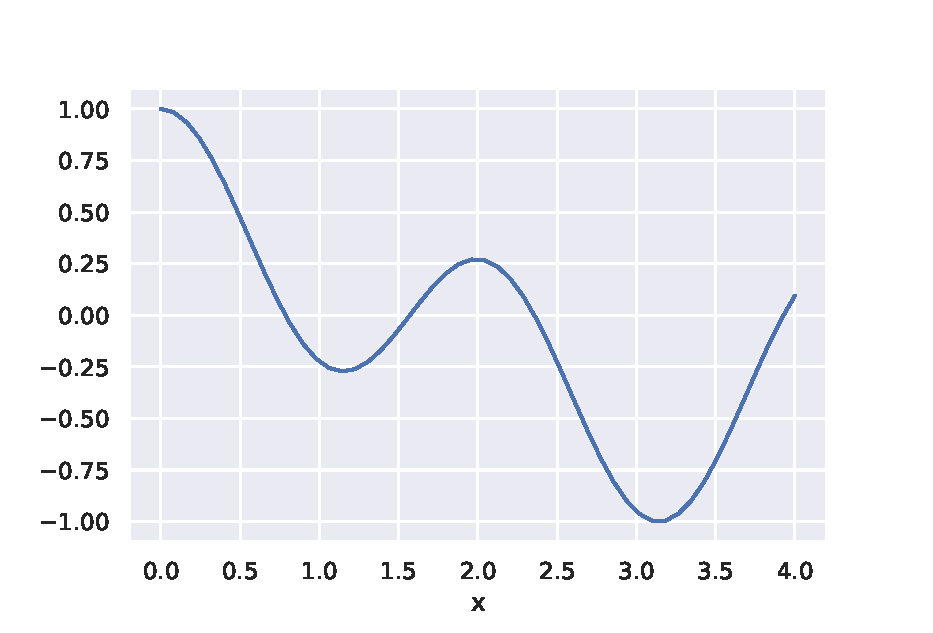
\includegraphics[width=0.7\linewidth]{figs/cos}
	\caption{}
	\label{fig:cos}
\end{figure}
\end{homeworkSection}


\pagebreak
\begin{homeworkSection}
\begin{lstlisting}[language=Python]
#centros de massas assumidos
y_1 = 3.0
y_2 = 3.4

X = np.array([0, 4, 6, 9])

Distances = np.vstack(((X - y_1)**2, (X - y_2)**2))
Prob = np.exp(-Distances) / np.sum(np.exp(-Distances), axis=0)
\end{lstlisting}
A matriz $p(y|x)$ é $\begin{bmatrix}
	0.92824246 & 0.34524654 & 0.09621554 & 0.00956532 \\ 
	0.07175754 & 0.65475346 & 0.90378446 & 0.99043468
\end{bmatrix} $.

\end{homeworkSection}



\begin{homeworkSection}
\begin{lstlisting}[language=Python]
D = np.sum(Distances*Prob)/len(X)
print(f'O valor de D é {D:.3}')
\end{lstlisting}
O valor de D é $12.0$.

\end{homeworkSection}

\begin{homeworkSection}
\begin{lstlisting}[language=Python]
y_1 = np.sum(Prob[0,:]*X.T)/np.sum(Prob[0,:])
y_2 = np.sum(Prob[1,:]*X.T)/np.sum(Prob[1,:])
print(f'O primeiro centroide y_1 é {y_1:.3}, o segundo y_2 é {y_2:.3}')

\end{lstlisting}
O primeiro centroide $y_1$ é $ 1.48 $, o segundo $y_2$ é $ 6.47 $.

\end{homeworkSection}



\begin{homeworkSection}
A matriz $p(y|x)$ é $\begin{bmatrix}
1 & 1.65880108e-03 & 0 & 0 \\ 
0 & 9.98341199e-01 & 1 & 1
\end{bmatrix} $. \\
O valor de D é $11.9$.
O primeiro centroide $y_1$ é $ 0.00662 $, o segundo $y_2$ é $ 6.33 $.	
\end{homeworkSection}



\begin{homeworkSection}
	A matriz $p(y|x)$ é $\begin{bmatrix}
	0.5127972 & 0.49680004 & 0.48880187 & 0.47681664 \\ 
	0.4872028 & 0.50319996 & 0.51119813 & 0.52318336
	\end{bmatrix} $. \\
	O valor de D é $13.1$.
	O primeiro centroide $y_1$ é $ 4.66 $, o segundo $y_2$ é $ 4.83 $.	
\end{homeworkSection}

\begin{homeworkSection}
	Quando a temperatura é alta, temos um "hard clustering", quando a temperatura é baixa, determínistico. O contrário, "soft clustering" acontece quando a temperatura é mais baixa.
\end{homeworkSection}

\end{homeworkProblem}




\begin{homeworkProblem}
	Vou usar a função
	\begin{equation}
	J(x_{0},x_1, \hdots, x_{19}) = \sum_{i = 9}^{19} V(x_{i})
	\end{equation}
	onde $V(x)$ é tal que
	\begin{equation}
	V(x) = \left[(x+1)x(x-1)\right]^{2} + 0.1x^{2}
	\end{equation}
Usamos temperaturas de $0.1$ até $0.01$. O único mínimo global é a origem.
\end{homeworkProblem}
O estado de menor custo encontrafo tinha custo 0.0312. O custo não é o mínimo, mas está bem próximo. O estado com menor custo satisfaz $|x_{i}| < 0.09$ em todas as coordenadas.

\end{document}